\subsection{Probabilistic Payments}

In traditional payment channels, two parties A and B lock some funds within a
smart contract, make transactions off-chain and only commit the aggregation
on-chain. Thus, a channel is bidirectional which means that both A and B can
send and receive transactions within the same channel. The HOPR protocol uses
unidirectional channels to implement bidirectional channel behavior where a channel is created from A to B and another from B to A. 
The channel creator is the sole owner of funds in the channel and the one able to create tickets. A channel created from
party $A$ to party $B$ is different from a channel created from party $B$ to
party $A$.

 $$A\rightarrow B \neq B\rightarrow A$$
This separation reflects the directional nature of packets flowing through the
network.
\\\textbf{Acknowledgements} are messages which allow every node to acknowledge the
processing of a packet to the previous node. This acknowledgement contains the
cryptographic material to unlock the possible payout for the previous node. Note
that acknowledgement is always sent to the previous node. In vanilla payment channels, the latest acknowledgement contains all previous incentives plus the incentive for the most recent interaction as explained below:

\begin{align}
value_(ACK_n) &=\sum_{i=1}^nfee_{packet_i}
\end{align}
where $n$ is the total number of mixnet packets transformed.
\\~\\If B received $ACK_n$ for $packet_n$ before sending $packet_{n-1}$, it has no
incentive to process $packet_{n-1}$ rather than $packet_{n}$. To avoid these
false incentives the HOPR protocol utilizes \textbf{probabilistic payments}.
In probabilistic payments the payouts use \textit{tickets} (further explained in
section \nameref{sec:tickets}). A ticket can be either a win or a loss with a
certain winning probability. This means nodes are incentivized to continue
relaying packets as they don’t know which ticket is a win. To a node each
ticket has the same value it is being claimed, thus the HOPR protocol
encourages nodes to claim tickets independently from each other.

\begin{align}
 value ( ACK_i )  &  =value ( ACK_j ) \quad for \quad i,j\in \{1,n\}
\end{align}
There is no added value in pretending packet loss or intentionally changing the order in which packets are processed.

\subsubsection{Channel Management}
Initially, each payment channel in HOPR is CLOSED which means that in order to transfer packets, those channels have to be opened. There are four distinct channel statuses which are represented in the following scheme:

\begin{figure}[H]
    \centering
    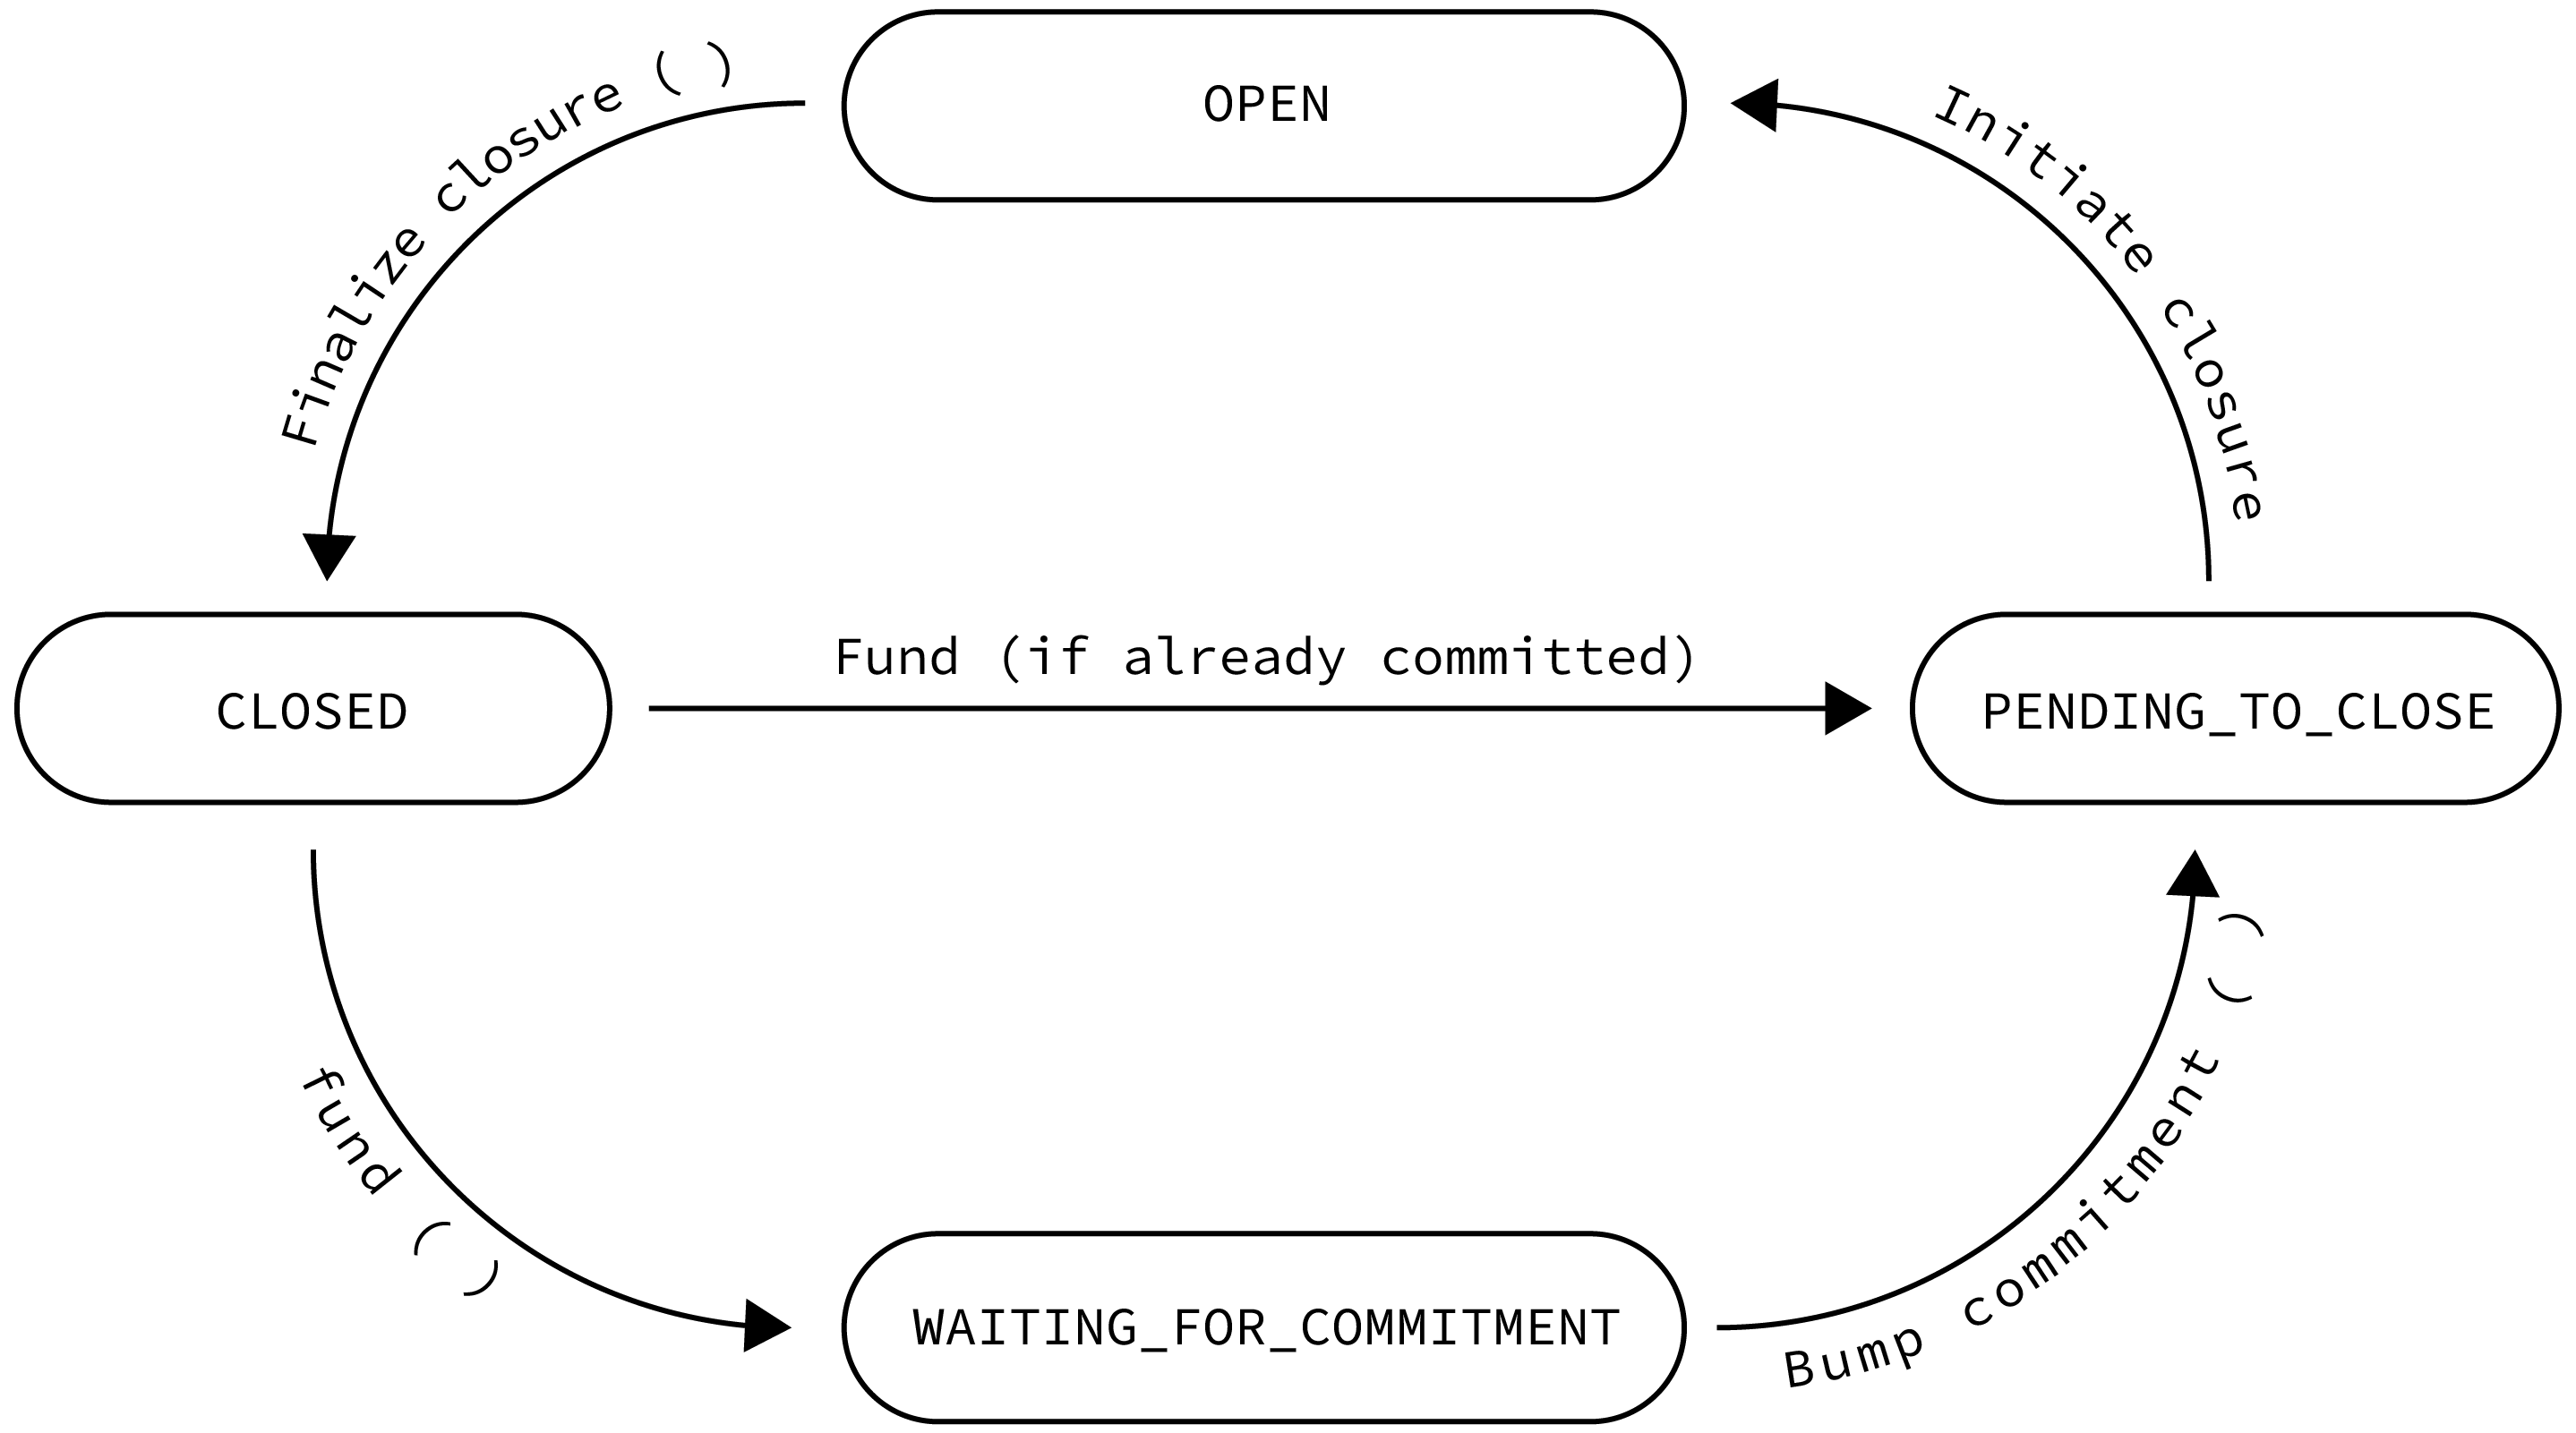
\includegraphics[width=9cm,height=9cm,keepaspectratio]{../yellowpaper/images/states1.png}
\label{fig:channel statuses}
    \caption{Channel statuses}
\end{figure}

\paragraph{Opening a channel} Nodes can OPEN channels to other nodes by the following:
A calls the method \textit{fundChannelMulti()} such that:
$$fundChannelMulti(A: <\lambda>, B:<\mu> )$$ where $\lambda$ and $\mu$ are the amounts to be staked by the sender A for A and B. Both values can also be equal or any of them could be zero. This function opens two unidirectional channels $A\rightarrow B$ and $B\rightarrow A$ if both staked amounts are specified. If not, only the channel $A\rightarrow B$ is opened where $A$ is the sender and $B$ is the recipient.
The channel is then on state \textit{WAITING\_FOR\_COMMITMENT}.
\\~\\The destination address of the channel must now commit in order for the channel between both parties to be open.
The channel destination (let's say it's B) can now call \textit{bumpChannel()} function to make a new set of commitments towards this channel. This call will trigger an onchain event \textit{ChannelIsOpened} and bumbs the ticket epoch to ensure tickets with the previous epoch are invalidated

\paragraph{Redeem tickets}
As long as the channel remains open, nodes can claim their incentives for forwarding packets which is represented as tickets (see ticket section). Tickets are redeemed by dispatching a \textit{redeemTicket()} call.
\\~\\If/when B tries to redeem a ticket from the channel $A\rightarrow B$ (spending channel) but also there is an open channel $B\rightarrow A$ (earning channel), B's rewards will go to $B\rightarrow A$. Otherwise, rewards will be sent directly to B.

\paragraph{Closing a channel}
Nodes can close a payment channel in order to access their funds. The way to do so is using a timeout.
Only the channel creator (let's say it's A) can initiate the process by calling \textit{initiateChannelClosure()}. This changes the state to $PENDING\_TO\_CLOSE$. Other nodes should monitor blockchain events to be aware of this change and thus will have now time to claim not yet claimed tickets.
\\~\\Once the timeout is done, (A) can call \textit{finalizeChannelClosure()} which turns the channel state into CLOSED. When channel is closed, funds (stake) are transfered automatically back to (A). Every ticket that wasn't redeemed while channel was open can't be redeemed after closure. This is guaranteed by using Channel Epoch which is explained in ticket section.

\begin{comment}

\begin{figure}[H]
    \centering
    \begin{tikzpicture}[looseness=1,auto]
        \path (0,0) node (closed) [ellipse,draw] {$Closed$};
        \path (-1,-1)  node (commitment) [ellipse,draw,align=left] {$Waiting$\\$Commitment$};
        \path (5,0)  node (open) [ellipse,draw] {$Open$};
        \path (2.5,-1)  node (pending) [ellipse,draw,align=left] {$Pending$\\$Timeout$};

        \draw [->,draw](closed) to [bend left] node {\textsf{fund()}} (commitment);
        \draw [->,draw](commitment) to [bend left] node {\textsf{fund()}} (open);
        \draw [->,draw](open) to [bend left] node [align=center] {\textsf{initiateChannelClosure()}} (pending);
        \draw [->,draw](pending) to [bend left] node {\textsf{finalizeChannelClosure()}} (closed);

        \path[->] (open) edge [out=+120,in=+60,distance=2em,below] node [align=center,above] {\textsf{redeemTicket()}}  (open);
    \end{tikzpicture}
    \label{fig:channel workflow}
    \caption{Channel workflow}
\end{figure}
\end{comment}

\begin{comment}
  \draw [->,draw](commitment) to [bend left] node {\textsf{fund()}} (open);
    \draw [->,draw](open) to [bend left] node [align=center] {\textsf{initiateChannelClosure()}} (pending);
    \draw [->,draw](pending) to [bend left] node {\textsf{finalizeChannelClosure()}} (closed);  
\end{comment}
